\documentclass[12pt,a4paper]{article}
\usepackage[UTF8]{ctex} % 支持中文
\usepackage{geometry}
\usepackage{graphicx}
\usepackage{amsmath}
\usepackage{float}
\usepackage{subfigure}
\usepackage{booktabs} % 表格美化
\usepackage{cite}
\usepackage{ulem}
\usepackage{array}
\usepackage{multirow}
\usepackage{hanging}


\newcolumntype{M}[1]{>{\centering\arraybackslash}m{#1}}
\newcommand{\down}[2]
{
	$\Delta_{\text{#1}}\approx{#2}$
}

% 设置页面边距
\geometry{left=2.5cm,right=2.5cm,top=2.5cm,bottom=2.5cm}

\title{\Huge{\textbf{\uuline{实\ 验\ 报\ 告}}}}
\author{\uline{少年班}\ 学院 \quad 姓名:\ \uline{顾泓宇} \quad 学号:\ \uline{PB23000078} \quad 实验日期:\ \uline{2024-3-18} }
\date{}

\begin{document}
	\maketitle
	
	\section{实验题目}
	单摆法测重力加速度
	
	\section{实验目的}
	采用单摆法测量了合肥的重力加速度，在 1\%的测量精度要求下利用不确定度分析对实验方案进行了设计，通过对周期的累积放大提高了测量精度。最终测得合肥的重力加速度为$9.76m/s^2$,其标准不确定度为$ $，满足实验的精度要求。调节单摆的摆长，测量了周期 T 随摆长 l 的变化，对 l 与 $T_{2}$ 的关系进行了线性拟合，求得了重力加速度。还通过视频追踪分析了大摆角情况下单摆的运动轨迹，研究了摆角和空气阻力对单摆周期的影响
	
	\section{实验仪器}
	钢卷尺、游标卡尺、千分尺、电子秒表、单摆（带标尺、平面镜；摆线长度可调，其可调的上限约为 100 cm）、智能手机（自备）、傅科摆、凯特摆。\\ 
	\hspace*{2em} 各测量仪器的最大允差如下：\\
	游标卡尺$\Delta_{\text{卡}}\approx0.002cm$；千分尺\down{千}{0.001cm}；秒表
	\down{秒}{0.05s}；\down{人}{0.2s}\\
	\hspace*{2em} 用钢卷尺测量单摆摆长时难以将被测物两端与测量仪器的刻线对齐，作为保守估计，一般可取不确定度\down{B}{0.2cm}; \\
	\hspace*{2em}
	开始实验前，应调节螺栓使立柱竖直，并调节标尺高度，使其上沿中点距
	悬挂点 50 cm。
	
	
	
	\section{实验原理}
	在本实验中，实验精度$\frac{\Delta g}{g}<1\%$,故摆球的几何形状、摆的质量、空气浮力、摆角等因素对
	测量造成的修正项均是高阶小量，可忽略。那么近似的周期测量公式为$T=2\pi\sqrt{\frac{L}{g}}$,故可通
	过不确定度均分原理，在一定的精度范围内测量T、L，从而求得重力加速度g。
	
	\section{实验设计}
	由$T=2\pi\sqrt{\frac{L}{g}}$，得$g=4\pi^2\frac{L}{T^2}$.由此得到不确定度合成公式$\frac{\Delta g}{g}=\sqrt{{(2\frac{\Delta T}{T})}^2+{(\frac{\Delta L}{L})}^2}$,若要求$\frac{\Delta g}{g}<1\%$,由不确定度均分原理，则有$2\frac{\Delta T}{nT}<0.5\%$和$\frac{\Delta L}{L}<0.5\%$，其中$n\in \mathbf{N}^*$,$\Delta T=\Delta_{\text{秒}}+\Delta_{\text{人}}\approx0.05s+0.2s=0.25s$，取$g\approx9.8m/s^2$,得到$T\approx1.68s$,代入$\frac{\Delta g}{g}=\sqrt{{(2\frac{\Delta T}{T})}^2+{(\frac{\Delta L}{L})}^2}<1\%$,解得$n\geq25$,则若一次测量要达到所需的精度，需要测量n=25个周期的时间. \\
	\hspace*{2em}
	除上述分析中提到的实验仪器外，还需要选择电子秒表、支架、细线、钢球。
	
	\section{实验步骤}
	1、按照实验要求组装好实验仪器，将电子秒表归零；\\
	\hspace*{2em}
	2、多次（本实验中 6 次）测量摆球直径、摆线长度；\\
	\hspace*{2em}
	3、将摆球拉离平衡位置使其小角度（小于 5 度）同平面摆动；\\
	\hspace*{2em}
	4、多次（本实验中 6 次）用电子秒表测量单摆 25 次全振动所需时间；\\
	\hspace*{2em}
	5、整理仪器；\\
	\hspace*{2em}
	6、数据处理和误差分析。\\
	
	\subsection{数据分析}
	实验所测量得到的结果如下：
	\begin{center}
		\begin{tabular}{|M{6em}|M{6em}|M{6em}|M{6em}|}\hline
			测量序号 & 摆线长度/cm & 摆球直径/mm & 25个周期全振动时间/s  \\\hline
			1 & 63.80 & 22.02 & 40.57  \\\hline
			2 & 63.70 & 22.00 & 40.40  \\\hline
			3 & 64.03 & 22.02 & 40.92  \\\hline
			4 & 63.97 & 22.02 & 40.91  \\\hline
			5 & 63.10 & 22.00 & 40.28 \\\hline
			6 & 63.12 & 22.02 & 40.44  \\\hline
		\end{tabular}
		\\表一：原始数据
	\end{center}
	摆长的平均值$\overline{l}=\frac{63.80+63.10+65.03+64.97+63.10+63.12}{6}cm=64.62cm$（摆球半径取为1cm）\\
	25个周期全振动时间的平均值$\overline{t}=\frac{40.57+40.40+40.92+40.91+40.28+40.44}{6}=40.59s$,则周期$T=\frac{t}{25}=1.62s$,代入计算得$\overline{g}=4\pi^2\frac{\overline{l}+1}{\overline{T}^2}=9.721m/s^2$
	\subsection{不确定度分析}
	1.摆长测量模型为:$l=l_{0}+l_{1}+l_{2}$,其中$l_{0}$为卷尺直接读出的长度，$l_{1}$为卷尺误差对测量结果的影响，$l_{2}$为使用卷尺测量摆长时难以完全对齐对测量结果的影响，考虑到测量精度要求，测量模型中忽略了其他因素的影响。\\
	由上述计算得，摆线长度的标准不确定度$u_{l_{0}}$为：\\
	$u_{l_{0}}=\sqrt{\frac{\sum_{i=1}^{n} (l_{i}-\overline{l})^2}{n(n-1)}}=0.106s$\\
	卷尺仪器误差造成的影响采用B类不确定度,卷尺最大允差为0.0012m，则其标准不确定度$u_{l_{1}}$为：\\
	$u_{l_{1}}=\frac{0.0012}{3}=0.4\times10^{-3}m$\\
	对于$l_{2}$,采用B类不确定度，由于未对齐产生偏差最大为0.2cm，则其标准不确定度为：
	$u_{l_{2}}=\frac{0.002}{3}=6.7\times10^{-4}m$\\
	故摆长的标准不确定度为：
	$u_{l}=\sqrt{u_{l_{0}}^2+u_{l_{1}}^2+u_{l_{2}}^2}=1.8\times10^{-3}m$\\
	\hspace*{2em}
	2.周期测量模型为:$T=\frac{t_{0}+t_{1}+t_{2}}{25}$,其中$t_{0}$为秒表时间，$t_{1}$为秒表仪器误差对测量的影响，$t_{2}$为人反应时间对测量的影响，考虑到测量精度要求，测量模型中忽略了其他因素的影响。\\
	由上述计算得，摆线长度的标准不确定度$u_{t_{0}}$为：\\
	$u_{t_{0}}=\sqrt{\frac{\sum_{i=1}^{n} (t_{i}-\overline{t})^2}{n(n-1)}}=0.106s$\\
	秒表仪器误差造成的影响采用B类不确定度,卷尺最大允差为0.05s，则其标准不确定度$u_{t_{1}}$为：\\
	$u_{t_{1}}=\frac{0.05}{3}=0.017s$\\
	人反应时间造成的影响采用B类不确定度，已知$\delta_{B}=0.2s$,则其标准不确定度$u_{t_{2}}$为：\\
	$u_{t_{2}}=\frac{0.2}{3}=0.067s$\\
	故摆长的标准不确定度为：
	$u_{T}=\sqrt{(\frac{1}{25})^2u_{t_{0}}^2+(\frac{1}{25})^2u_{t_{1}}^2+(\frac{1}{25})^2u_{t_{2}}^2}=0.00506s$\\
	\hspace*{2em}
	3.代入重力加速度不确定度公式得g的标准不确定度为$0.0664m/s^2$,相对不确定度为$0.683\%$,小于1\%，满足精度要求。
	\section{提升内容}
		\begin{center}
			\begin{tabular}{|M{6em}|M{6em}|M{6em}|M{6em}|}\hline
			测量序号 & 摆线长度/cm & 25个周期全振动时间/s & $T^2$/$s^2$   \\\hline
			1 & 54.91 & 37.50 & 2.2500  \\\hline
			2 & 59.72 & 39.14 & 2.4511  \\\hline
			3 & 62.31 & 40.05 & 2.5664  \\\hline
			4 & 64.43 & 40.70 & 2.6504  \\\hline
			5 & 67.60 & 41.11 & 2.7041  \\\hline
			6 & 71.91 & 43.13 & 2.9763  \\\hline
			\end{tabular}
		\\表二：原始数据\\
		(注:摆球半径取为1cm)\\
			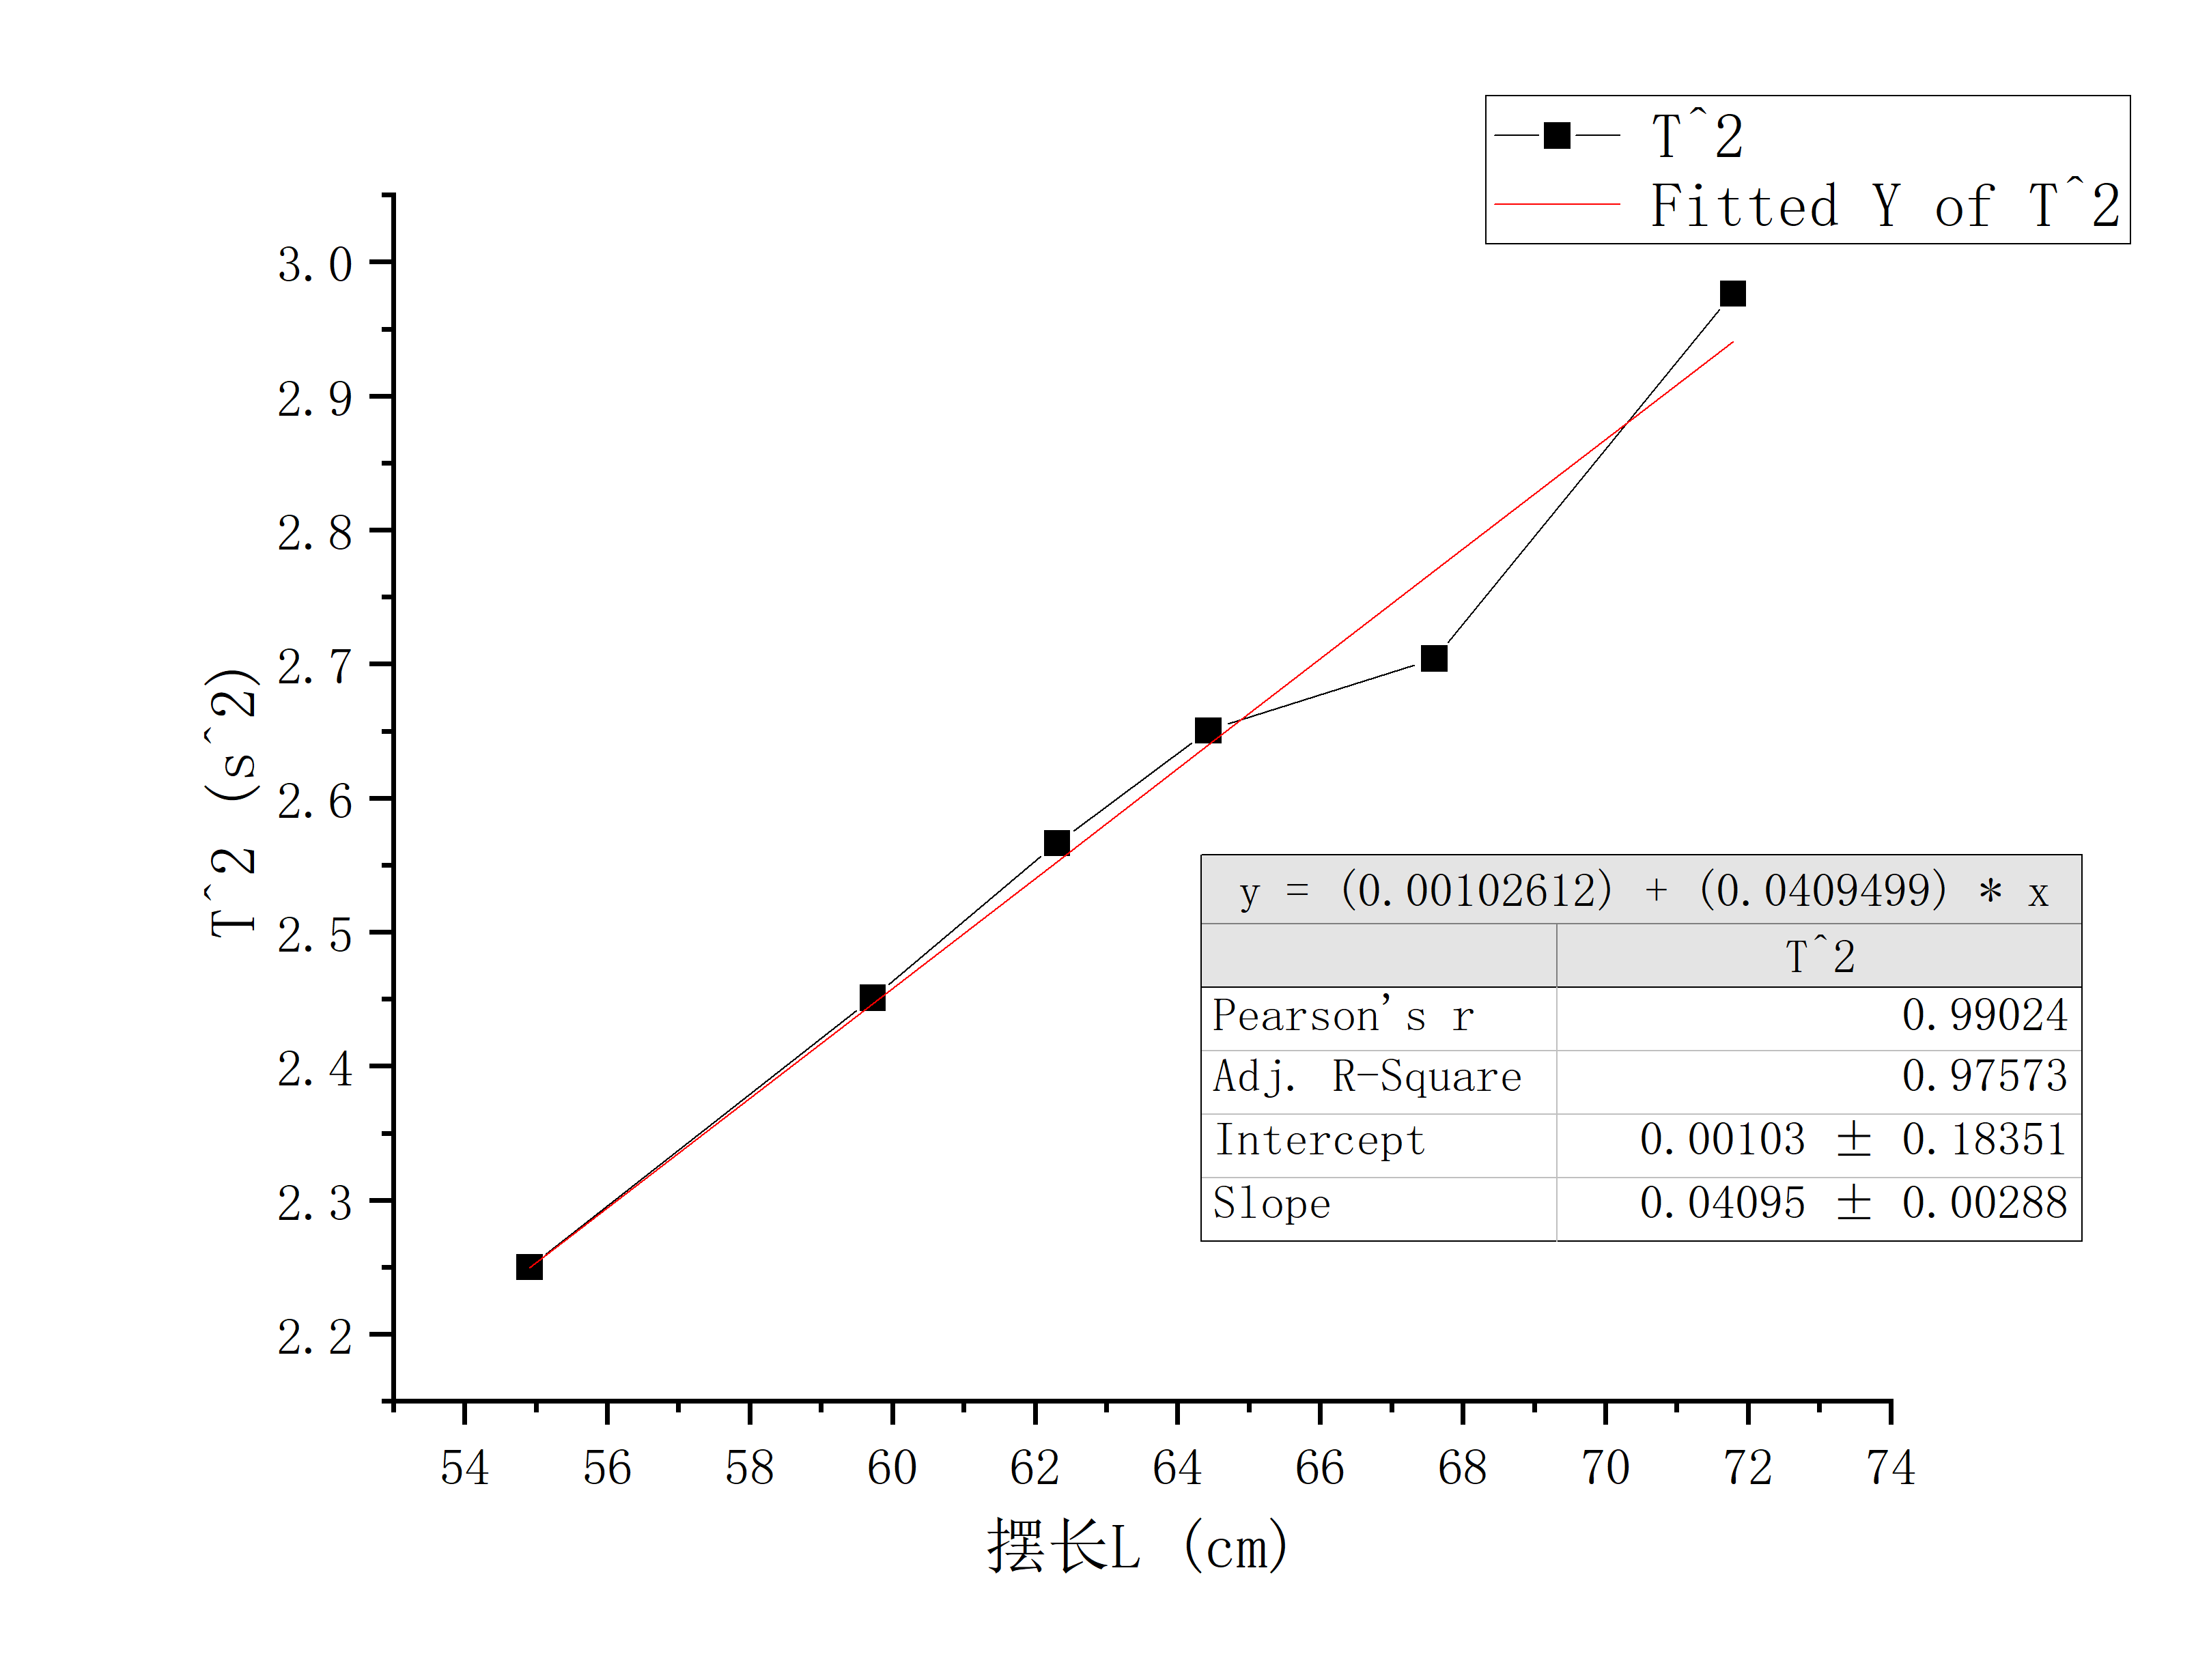
\includegraphics[width=0.8\textwidth]{单摆.png}\\
	\end{center}
	根据最小二乘法的拟合结果，如图拟合函数为$T^2=0.00102612+0.0409499\times L$,计算得$g=\frac{4\pi^2 \times 10^{-2}}{0.0409499}\approx9.65m/s^2$,其标准不确定度为$u_{g}=4\pi^2\times u_{k}=0.113m/s^2$,相对不确定度为$0.10\%$，满足精度要求。
	\section{进阶内容}
		利用智能手机录制单摆视频。用视频追踪技术（Tracker）获取单摆的运动轨迹，研究摆角为$10 ^\circ$条件下单摆的运动规律。对运动轨迹数据进行拟合分析。以下是运动的x-t和y-t图像及坐标轴位置：\\
		\begin{center}
			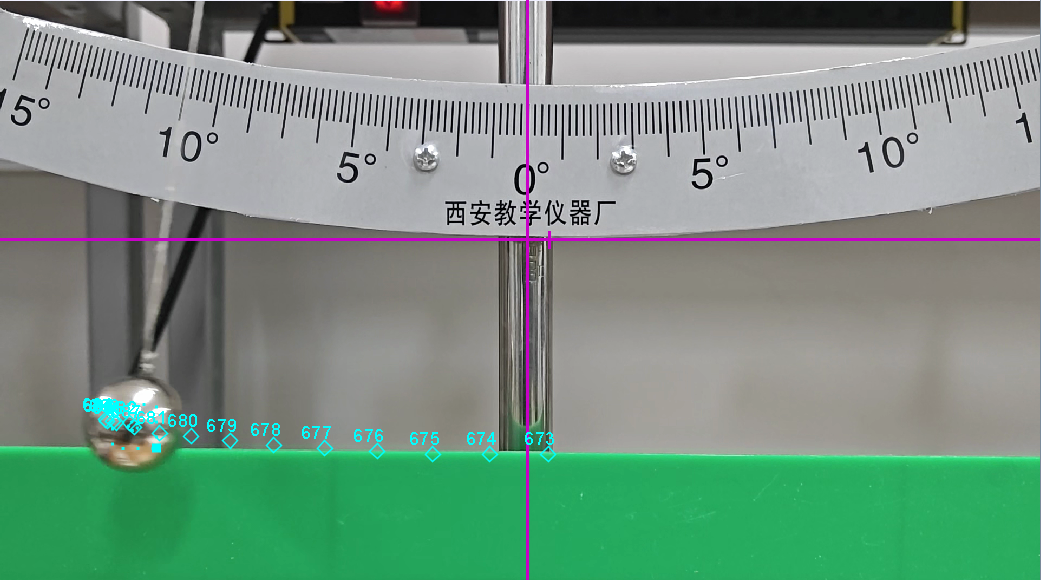
\includegraphics[width=0.8\textwidth]{track1.png}\\
			图一：拟合坐标轴位置\\
			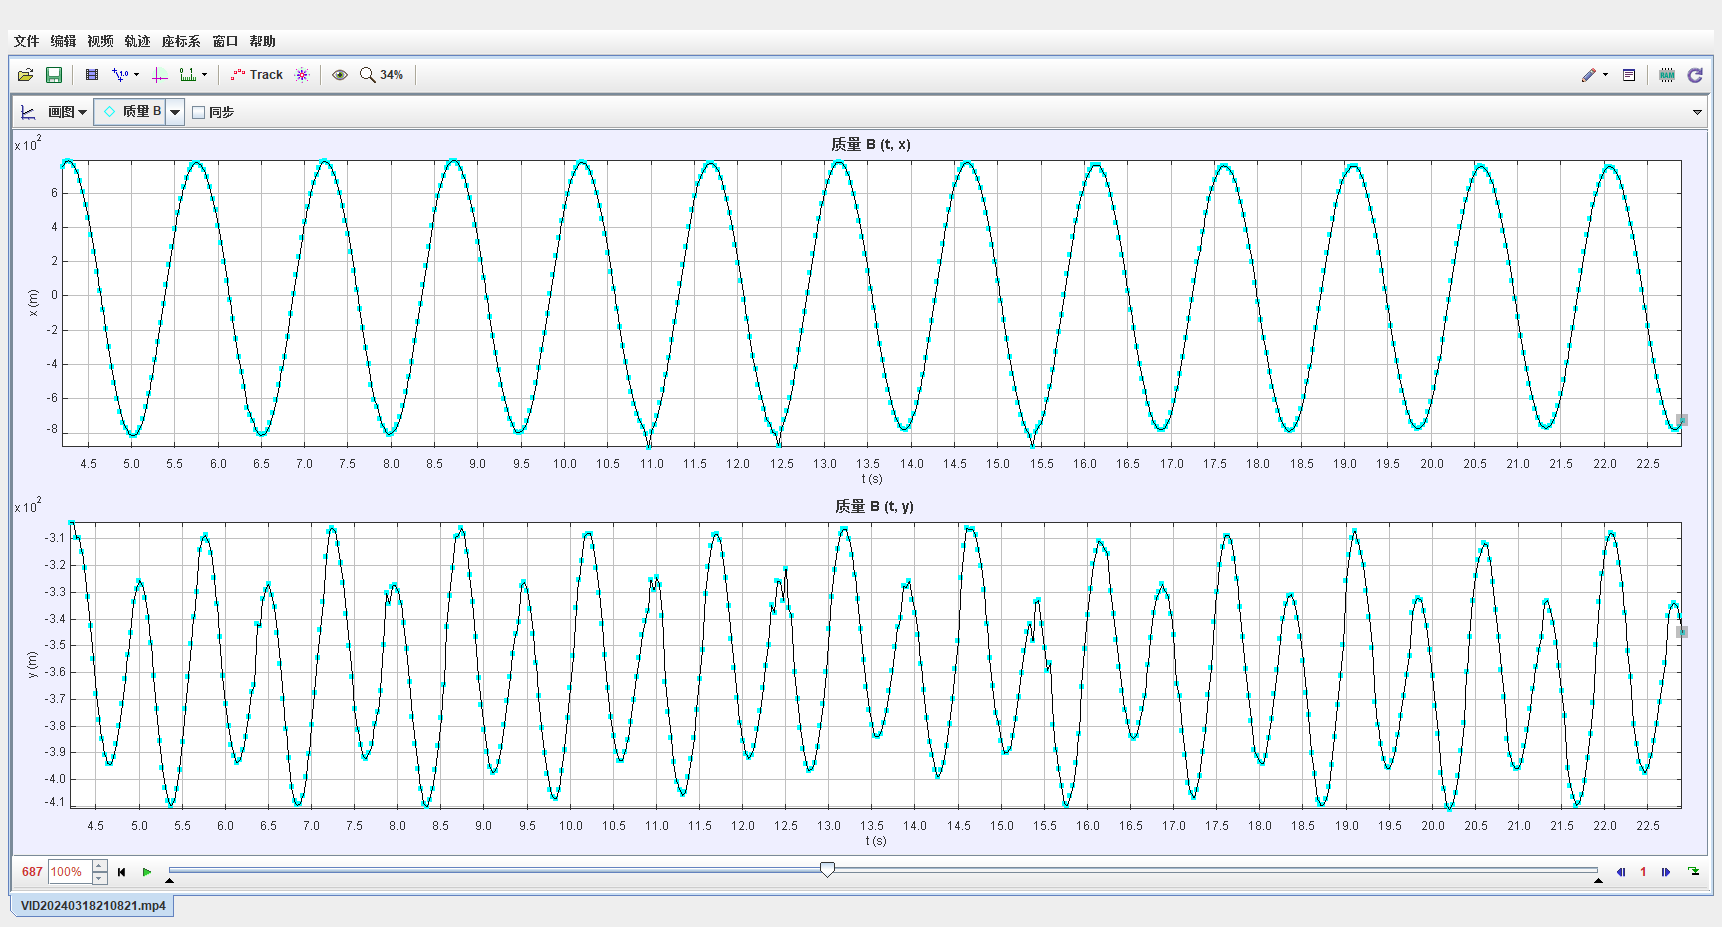
\includegraphics[width=0.8\textwidth]{tracker1.png}\\
			图二：运动的x-t及y-t图像\\
		\end{center}
		拟合结果给出单摆的摆动周期T为1.632s,测的单摆摆长为0.657m,代入未修正的重力加速度公式得：\\
		\begin{center}
			g=$\frac{4\pi^2l}{T^2}=9.738m/s^2$
		\end{center}
		如果考虑大摆角的修正，则重力加速度为：
		\begin{center}
			g=$\frac{4\pi^2l}{T^2}(1+\frac{1}{4}\sin^2(\frac{\theta}{2}))^2=9.775m/s^2$
		\end{center}		
		可以看出修正后的结果与合肥的重力加速度参考值$9.795m/s^2$更为接近。
	\section{结论}
	本实验用三种方法测得的合肥地区重力加速度分别为9.721$m/s^2$,9.65$m/s^2$，9.775$m/s^2$与参考值9.795$m/s^2$的偏差均小于1\%, 在10°的大摆角情况下研究了摆角和空气阻力对单摆周期的影响，结果表明考虑摆角修正后测得的重力加速度更接近参考值，修正对测量结果的影响约为0.37\%
	
	\section{参考文献}
	[1]. 单摆法测重力加速度. 实验讲义.2024
	
\end{document}